\newpage
\chapter{Lagerlebensdauerberechnung}
\section{Lagerkräfte im Gang 1}
\subsubsection{Berechnung der Zahnradkräfte}
Die Berechnung der Kräfte und die verwendeten Formeln entsprechen dem Kapitel 3.2. Im 1. Gang sind Z1/Z2 und Z6/Z7 im Eingriff.
\begin{itemize}
\item Gegebene Werte: 
	\begin{align*}
	&n_{\mathrm{II},1} = 400\frac{1}{\text{min}} \\
	&T_{\mathrm{II},1,S} = 18,4\text{ Nm} \\
	&T_{\mathrm{III},1,S} = 73,63\text{ Nm} \\	
	&d_2 = 217,1\text{ mm} \text{ , } d_6 = 149 \text{ mm , } d_8 = 112 \text{ mm}
	\end{align*}
\item Z2, Gang 1:
	\begin{align*} 
	&F_{t,2,1} = \frac{2\x T_{\mathrm{II},1,S}}{d_2} = \frac{2 \x 18,4 \text{ Nm}}{0,2171 \text{ m}} = 169,5 \text{ N}\\ 
	&F_{r,2,1} = \frac{169,5 \text{ N} \x \tan{(20^\circ)}}{\cos(20^\circ)} = 65,65\text{ N}\\ 
	&F_{a,2,1} =169,5 \x \tan(20^\circ) =61,7 \text{ N}
	\end{align*}
\item Z8, Gang 1:
	\begin{align*}
	&F_{t,8,1} = \frac{2\x T_{\mathrm{II},1,S}}{d_8 \x 4} = \frac{2 \x 18,4 \text{ Nm}}{0,112 \text{ m} \x 4} = 328,57\text{ N}\\ 
	&F_{r,8,1} = 328,57 \text{ N} \x \tan{(20^\circ)} = 115,59\text{ N}\\ 
	&F_{a,8,1} =0 \text{ N}
	\end{align*}
\item Z6, Gang 1:
	\begin{align*} 
	&F_{t,6,1} = \frac{2\x T_{\mathrm{III},1,S}}{d_6} = \frac{2 \x 73,63 \text{ Nm}}{0,149 \text{ m}} = 988,32 \text{ N}\\ 
	&F_{r,6,1} = \frac{988,32 \text{ N} \x \tan{(20^\circ)}}{\cos(20^\circ)} = 382,8\text{ N}\\ 
	&F_{a,6,1} =988,32 \x \tan(20^\circ) =359,72 \text{ N}
	\end{align*}
\end{itemize}
\subsubsection{Berechnung der Lagerkräfte}
\begin{itemize}
\item Momentensummen Hohlwelle:
\begin{center}
	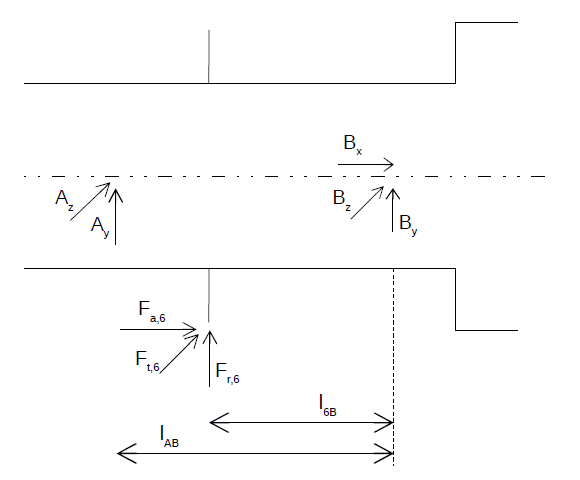
\includegraphics[width=1\textwidth,keepaspectratio]{figures/Gang1Hohl.png}
\end{center}
\[l_{AB} =171\text{ mm} \text{ , } l_{6B} = 128,5\text{ mm}\]
\begin{align*}
	\sum M\textsubscript{y}\textsuperscript{(B)} &\overset{!}{=} 0 = -A_z \x l_{AB} - F_{t,6,1} \x l_{6B} \\
	&\implies A_z = -F_{t,6,1} \x \frac{l_{6B}}{l_{AB}} = -742,68 \text{ N} \\ \\
	\sum M\textsubscript{z}\textsuperscript{(B)} &\overset{!}{=} 0 = -A_y \x l_{AB} - F_{r,6,1} \x l_{6B} + F_{a,6,1} \x \frac{d_6}{2}\\
	&\implies A_y = \frac{-F_{r,6,1} \x l_{6B} + F_{a,6,1} \x \frac{d_6}{2}} {l_{AB}}= -130,9 \text{ N} 
\end{align*}
\newpage
\item Gleichgewichte Welle II:
\begin{center}
	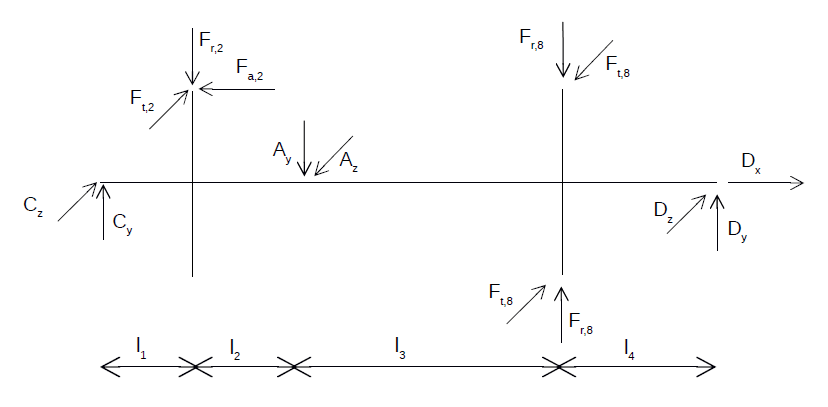
\includegraphics[width=1.04\textwidth,keepaspectratio]{figures/Gang1.png}
\end{center}
\begin{align*}
&l_{1} =269,5\text{ mm} \text{ , } l_{2} = 75,5\text{ mm} \text{ , } l_{3} = 273\text{ mm}  \text{ , } l_{4} = 47\text{ mm} \text{ , } l_{ges} = 665\text{ mm}
\end{align*}
\begin{align*}
	\sum F_x &\overset{!}{=} 0 = -F_{a,2,1} + D_x \implies D_x = F_{a,2,1} = 61,7 \text{ N} \\
	\sum F_y &\overset{!}{=} 0 = C_y - F_{r,2,1}-A_y +D_y - F_{r,8} + F_{r,8}\\ 
	\sum F_z &\overset{!}{=} 0 = A_z - C_z - D_z - F_{t,2,1} + F_{t,8} - F_{t,8}\\ \\
	\sum M\textsubscript{y}\textsuperscript{(D)} &\overset{!}{=} 0 = A_z \x (l_3+l_4)- F_{t,2,1} \x (l_2+l_3+l_4) - C_z \x l_{ges} +l_4 \x F_{t,8}- l_4 \x F_{t,8} \\ 
	&\implies C_z = \frac{(l_3+l_4) \x A_z - F_{t,2,1} \x (l_2+l_3+l_4)}{l_{ges}} = -458,2 \text { N} \\ 
	& \implies D_z = A_z - C_z - F_{t,2,1}= -454 \text{ N}\\ \\
	\sum M\textsubscript{z}\textsuperscript{(D)} &\overset{!}{=} 0 = (l_3+l_4) \x A_y + \frac{d_2}{2} \x F_{a,2,1} + (l_2+l_3+l_4) \x F_{r,2,1}- l_{ges} \x C_y  \\ 
	&\implies C_y = \frac{(l_3+l_4) \x A_y + \frac{d_2}{2} \x F_{a,2,1} + (l_2+l_3+l_4) \x F_{r,2,1}}{l\textsubscript{ges}} = -13,87 \text{ N}\\ 
	& \implies D_y =   A_y - C_y + F_{r,2,1} = -51,38\text{ N}
\end{align*}
\begin{align*}
	C_{x,1} &= \underline{0\text{ N}} & D_{x,1}= \underline{61,7\text{ N}}\\
	C_{y,1} &= \underline{-13,87\text{ N}} & D_{y,1}= \underline{-51,38\text{ N}}\\
	C_{z,1} &= \underline{-458,2\text{ N}} & D_{z,1}= \underline{-454\text{ N}}
\end{align*}
\end{itemize}
\section{Lagerkräfte im Gang 2}
\subsubsection{Berechnung der Zahnradkräfte}
Die Berechnung der Kräfte und die verwendeten Formeln entsprechen dem Kapitel 3.2. Im 2. Gang sind Z1/Z2 und Z4/Z5 im Eingriff.
\begin{itemize}
\item Gegebene Werte: 
	\begin{align*}
	&n_{\mathrm{II},2} = 400\frac{1}{\text{min}} \\
	&T_{\mathrm{II},2,S} = 48,96\text{ Nm} \\
	&d_2 = 217,1\text{ mm} \text{ , } d_4 = 89,4 \text{ mm } 
	\end{align*}
\item Z2, Gang 2:
	\begin{align*} 
	&F_{t,2,2} = \frac{2\x T_{\mathrm{II},2,S}}{d_2} = \frac{2 \x 48,96 \text{ Nm}}{0,2171 \text{ m}} = 451 \text{ N}\\ 
	&F_{r,2,2} = \frac{451 \text{ N} \x \tan{(20^\circ)}}{\cos(20^\circ)} = 174,7\text{ N}\\ 
	&F_{a,2,2} =451 \x \tan(20^\circ) =164,15 \text{ N}
	\end{align*}
\item Z4, Gang 2:
	\begin{align*} 
	&F_{t,4,2} = \frac{2\x T_{\mathrm{II},2,S}}{d_4} = \frac{2 \x 48,96 \text{ Nm}}{0,0894 \text{ m}} = 1095,3 \text{ N}\\ 
	&F_{r,4,2} = \frac{1095,3 \text{ N} \x \tan{(20^\circ)}}{\cos(20^\circ)} = 424,2\text{ N}\\ 
	&F_{a,4,2} =1095,3 \x \tan(20^\circ) =398,7 \text{ N}
	\end{align*}
\end{itemize}
\newpage
\subsubsection{Berechnung der Lagerkräfte}
\begin{itemize}
	\item Gleichgewichte Welle II:
	\begin{center}
		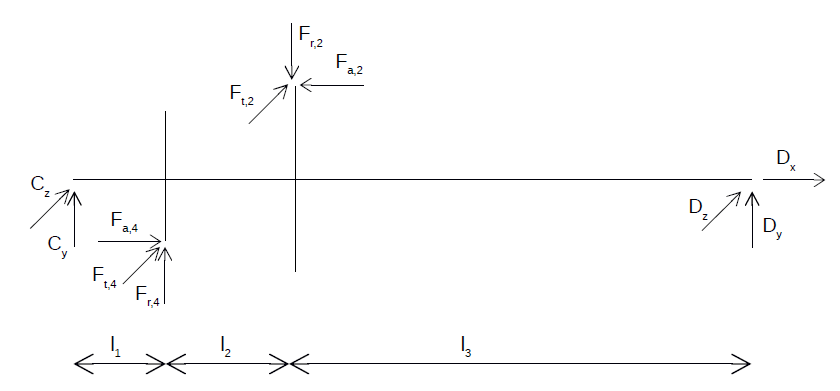
\includegraphics[width=1.04\textwidth,keepaspectratio]{figures/Gang2.png}
	\end{center}
\[l_{1} =118\text{ mm} \text{ , } l_{2} = 151,5\text{ mm} \text{ , } l_{3} = 395,5\text{ mm}  \text{ , } l_{ges} = 665\text{ mm}\]
	\begin{align*}
	\sum F_x &\overset{!}{=} 0 = F_{a,4,2} -F_{a,2,2} + D_x \implies D_x = -F_{a,4,2} +F_{a,2,2}= -234,55 \text{ N} \\
	\sum F_y &\overset{!}{=} 0 = C_y +F_{r,4,2}- F_{r,2,2}+D_y \\ 
	\sum F_z &\overset{!}{=} 0 = - C_z - D_z - F_{t,2,2} - F_{t,4,2} \\ \\
	\sum M\textsubscript{y}\textsuperscript{(D)} &\overset{!}{=} 0 = - F_{t,2,2} \x l_3 - C_z \x l_{ges} -(l_2 + l_3) \x F_{t,4,2} \\ 
	&\implies C_z = \frac{- F_{t,2,2} \x l_3 - (l_2+l_3) \x F_{t,4,2} }{l_{ges}} = -1169,2 \text { N} \\ 
	& \implies D_z = - C_z - F_{t,2,2} - F_{t,4,2}= -377,1 \text{ N}\\ \\
	\sum M\textsubscript{z}\textsuperscript{(D)} &\overset{!}{=} 0 = \frac{d_2}{2} \x F_{a,2,2} + \frac{d_4}{2} \x F_{a,4,2} + l_3 \x F_{r,2,2} - (l_2 + l_3) \x F_{r,4,2}- l_{ges} \x C_y  \\ 
	&\implies C_y = \frac{ \frac{d_2}{2} \x F_{a,2,2} + \frac{d_4}{2} \x F_{a,4,2}  + l_3 \x F_{r,2,2} - (l_2 + l_3) \x F_{r,4,2}}{l\textsubscript{ges}} = -191,6 \text{ N}\\ 
	& \implies D_y =  - C_y - F_{r,4,2} + F_{r,2,2} = -58,1\text{ N}
	\end{align*}
	\begin{align*}
	C_{x,2} &= \underline{0\text{ N}} & D_{x,2}= \underline{-234,55\text{ N}}\\
	C_{y,2} &= \underline{-191,6\text{ N}} & D_{y,2}= \underline{-58,1\text{ N}}\\
	C_{z,2} &= \underline{-1169,2\text{ N}} & D_{z,2}= \underline{-377,1\text{ N}}
	\end{align*}
\end{itemize}
\section{Lagerkräfte im Gang 3}
\subsubsection{Berechnung der Zahnradkräfte}
Die Berechnung der Kräfte und die verwendeten Formeln entsprechen dem Kapitel 3.2. Im 3. Gang sind Z1/Z3 und Z6/Z7 im Eingriff.
\begin{itemize}
	\item Gegebene Werte: 
	\begin{align*}
	&n_{\mathrm{II},3} = \frac{n_{\mathrm{III},3}}{i_{9,8}} = 1600\frac{1}{\text{min}} \\
	&T_{\mathrm{III},3,S} = 121,63\text{ Nm} \\	
	&d_3 = 217,1\text{ mm} \text{ , } d_6 = 149 \text{ mm } 
	\end{align*}
	\item Z3, Gang 3:
	\begin{align*} 
	&F_{t,3,3} = \frac{2\x T_{\mathrm{III},3,S}}{d_3} = \frac{2 \x 121,63 \text{ Nm}}{0,2171 \text{ m}} = 1120,5 \text{ N}\\ 
	&F_{r,3,3} = \frac{1120,5 \text{ N} \x \tan{(20^\circ)}}{\cos(20^\circ)} =434\text{ N}\\ 
	&F_{a,3,3} =1120,5 \x \tan(20^\circ) =407,8 \text{ N}
	\end{align*}
	\item Z6, Gang 3:
	\begin{align*}
	&F_{t,6,3} = \frac{2\x T_{\mathrm{III},3,S}}{d_6} = \frac{2 \x 121,63 \text{ Nm}}{0,149 \text{ m}} = 1632,6\text{ N}\\ 
	&F_{r,6,3} = 1632,6 \text{ N} \x \tan{(20^\circ)} = 632,35\text{ N}\\ 
	&F_{a,6,3} =1632,6\x \tan(20^\circ) =594,2 \text{ N}
	\end{align*}
\end{itemize}
\newpage
\subsubsection{Berechnung der Lagerkräfte}
\begin{itemize}
	\item Momentensummen Hohlwelle:
	\begin{center}
		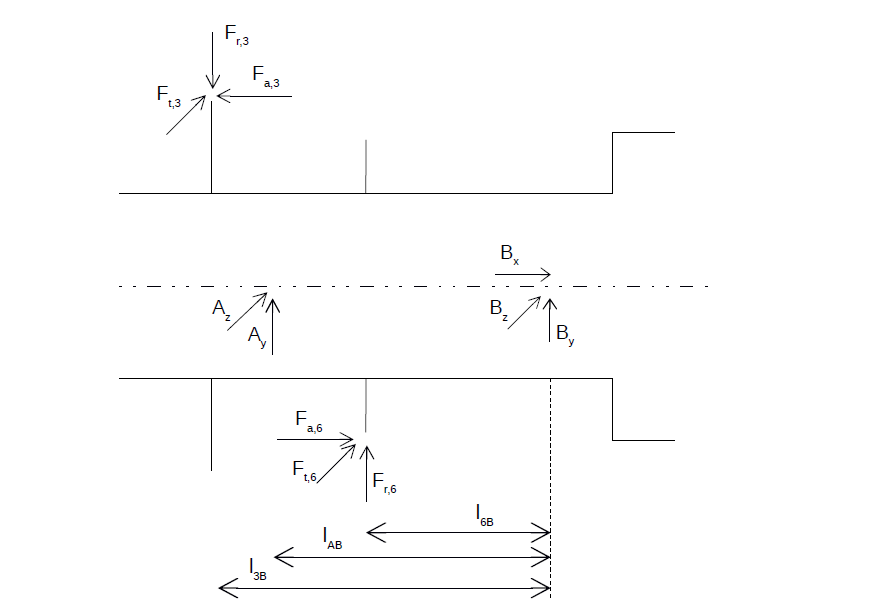
\includegraphics[width=1.2\textwidth,keepaspectratio]{figures/Gang3Hohl.png}
	\end{center}
\[l_{AB} =171\text{ mm} \text{ , } l_{3B} = 175,8\text{ mm} \text{ , } l_{6B} = 128,5\text{ mm}  \]
	\begin{align*}
	\sum M\textsubscript{y}\textsuperscript{(B)} &\overset{!}{=} 0 = -A_z \x l_{AB} - F_{t,6,3} \x l_{6B} - F_{t,3,3} \x l_{3B} \\
	&\implies A_z =  \frac{-F_{t,6,1} \x l_{6B} - F_{t,3,3} \x l_{3B}}{l_{AB}} = -2378,8\text{ N} \\ \\
	\sum M\textsubscript{z}\textsuperscript{(B)} &\overset{!}{=} 0 = -A_y \x l_{AB} - F_{r,6,3} \x l_{6B} + F_{a,6,3} \x \frac{d_6}{2} + F_{a,3,3} \x \frac{d_3}{2} + F_{r,3,3} \x l_{3B}\\
	&\implies A_y = \frac{-F_{r,6,3} \x l_{6B} + F_{a,6,3} \x \frac{d_6}{2} +F_{a,3,3} \x \frac{d_3}{2} + F_{r,3,3} \x l_{3B}} {l_{AB}}= 488,7 \text{ N} 
	\end{align*}
	\newpage
	\item Gleichgewichte Welle II:
	\begin{center}
		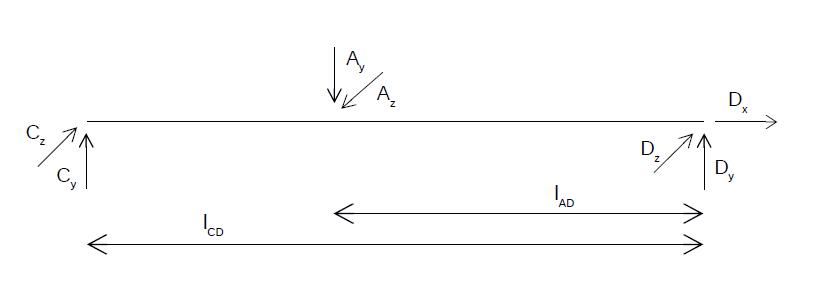
\includegraphics[width=1.04\textwidth,keepaspectratio]{figures/Gang3.png}
	\end{center}
\[l_{AD} =322\text{ mm} \text{ , } l_{CD} = 665\text{ mm} \]
	\begin{align*}
	\sum F_x &\overset{!}{=} 0 =  D_x \implies D_x =  0 \text{ N} \\
	\sum F_y &\overset{!}{=} 0 = C_y -A_y +D_y \\ 
	\sum F_z &\overset{!}{=} 0 = A_z - C_z - D_z\\ \\
	\sum M\textsubscript{y}\textsuperscript{(D)} &\overset{!}{=} 0 = A_z \x l_{AD} - C_z \x l_{CD}\\ 
	&\implies C_z = A_z \x \frac{l_{AD}}{l_{CD}} = -1151,8 \text { N} \\ 
	& \implies D_z = A_z - C_z = -1227 \text{ N}\\ \\
	\sum M\textsubscript{z}\textsuperscript{(D)} &\overset{!}{=} 0 = A_y \x l_{AD} - C_y \x l_{CD} \\ 
	&\implies C_y = A_y \x \frac{l_{AD}}{l_{CD}} = 236,6 \text{ N}\\ 
	& \implies D_y =   A_y - C_y = 252,1\text{ N}
	\end{align*}
	\begin{align*}
	C_{x,3} &= \underline{0\text{ N}} & D_{x,3}= \underline{0\text{ N}}\\
	C_{y,3} &= \underline{236,6\text{ N}} & D_{y,3}= \underline{252,1\text{ N}}\\
	C_{z,3} &= \underline{-1151,8\text{ N}} & D_{z,3}= \underline{-1227\text{ N}}
	\end{align*}
\end{itemize}
\section{Lagerkräfte im Gang 4}
Die Lagerkräfte der Welle 2 im 4. Gang wurden im Kaptel 3.2 zur Berechnung der Schnittkräfte bestimmt.
\begin{align*}
	n_{\mathrm{II},4} &= 1600\frac{1}{\text{min}} \\
	C_{x,4} &= \underline{0\text{ N}} & D_{x,4}= \underline{-581,94\text{ N}}\\
	C_{y,4} &= \underline{327,26\text{ N}} & D_{y,4}= \underline{710,23\text{ N}}\\
	C_{z,4} &= \underline{-2616,8\text{ N}} & D_{z,4}= \underline{-1689,53\text{ N}}
\end{align*}
\section{Berechnung der äquivalenten dynamischen Lagerbelastung}
Die Formeln für die Berechnung stammen aus dem Skript KL III\ccite{bib:poll:kl3} Seite 73 bis 74.
Die Werte für die statische und dynamisch Tragzahl stammen aus dem Tabellenbuch Roloff/Matek \ccite{bib:roloffMatek:tabellenbuch} Seite 205.
\subsection{Gang 1}
\subsubsection{Gang 1, Festlager:} Rillenkugellager , DIN 625-6206\\
\begin{itemize}
	\item gegebene Werte:
	\begin{align*}
	&n_{{\mathord{\mathrm{II}},1}} &&=  400 \frac{1}{\text{min}} \\
	&\text{statische Tragzahl } C_{0} &&= 11200 \text{ N}\\
	&\text{dynamische Tragzahl } C &&= 19300 \text{ N} \\
	&\text{Lebensdauerexponent } p &&= 3 \text{ (für Wälzlager)} \\
	&F_{Dx} && = 61,7 \text{ N}\\
	&F_{Dy} && = -51,38 \text{ N}\\
	&F_{Dz} && = -454 \text{ N}
	\end{align*} 
	\item Berechnung der äquivalenten dynamischen Belastung
	\begin{align*}
	&\text{dynamische radiale Lagerkraft } F_r&& = \sqrt{F_{Dy}^2 + F_{Dz}^2 } = 456,9 \text{ N} \\
	&\text{dynamische axiale Lagerkraft } F_a&& = |F_{Dx}| = 61,7 \text{ N}\\
	&\text{Belastungsfaktor } e &&= 0,22 \text{ da } \frac{F_a}{C_0} < 0,025
	\end{align*} 
	\[\frac{F_a}{F_r} = 0,14 \implies \frac{F_a}{F_r} < e\]
	Deshalb folgt aus Tabelle 2.9 im Skript KL III\ccite{bib:poll:kl3} : X= 1 \text{, } Y= 0 \\
	Die äquivalente dynamische Belastung ergibt sich zu: 
	\[
	P= X \x F_r = 456,9 \text{ N}
	\]
\end{itemize}

\subsubsection{Gang 1, Loslager:} Rillenkugellager, DIN 625-6206\\
\begin{itemize}
	\item gegebene Werte:
	\begin{align*}
	&n_{{\mathord{\mathrm{II}},1}} &&=  400 \frac{1}{\text{min}} \\
	&\text{statische Tragzahl } C_{0} &&= 11200 \text{ N}\\
	&\text{dynamische Tragzahl } C &&= 19300 \text{ N} \\
	&\text{Lebensdauerexponent } p &&= 3 \text{ (für Wälzlager)} \\
	&F_{Cy} && = -13,87 \text{ N}\\
	&F_{Cz} && = -458,2 \text{ N}
	\end{align*} 
	\item Berechnung der äquivalenten dynamischen Belastung
	\begin{align*}
	&\text{dynamische radiale Lagerkraft } F_r&& = \sqrt{F_{Cy}^2 + F_{Cz}^2 } = 458,4 \text{ N} \\
	&\text{dynamische axiale Lagerkraft } F_a&& = F_{Cx} = 0\text{ N}
	\end{align*} 
	Da es sich um eine reine Radialbelastung handelt, ergeben sich der Radial- und Axialfaktor zu: $X= 1$ und $Y=0$\\
	Daraus ergibt sich die äquivalente dynamische Lagerbelastung zu:  
	\[
	P= X \x F_r =458,4 \text{ N}
	\]
\end{itemize}
\newpage

\subsection{Gang 2}
\subsubsection{Gang 2, Festlager:} Rillenkugellager , DIN 625-6206\\
\begin{itemize}
	\item gegebene Werte:
	\begin{align*}
	&n_{{\mathord{\mathrm{II}},2}} &&=  400 \frac{1}{\text{min}} \\
	&\text{statische Tragzahl } C_{0} &&= 11200 \text{ N}\\
	&\text{dynamische Tragzahl } C &&= 19300 \text{ N} \\
	&\text{Lebensdauerexponent } p &&= 3 \text{ (für Wälzlager)} \\
	&F_{Dx} && = -234,55 \text{ N}\\
	&F_{Dy} && = -58,1 \text{ N}\\
	&F_{Dz} && = -377,1 \text{ N}
	\end{align*} 
	\item Berechnung der äquivalenten dynamischen Belastung
	\begin{align*}
	&\text{dynamische radiale Lagerkraft } F_r&& = \sqrt{F_{Dy}^2 + F_{Dz}^2 } = 381,5 \text{ N} \\
	&\text{dynamische axiale Lagerkraft } F_a&& = |F_{Dx}| = 234,55 \text{ N}\\
	&\text{Belastungsfaktor } e &&= 0,37 \text{ da } \frac{F_a}{C_0} = 0,02
	\end{align*}
	\[\frac{F_a}{F_r} = 0,6 \implies \frac{F_a}{F_r} > e\]
	Deshalb folgt aus Tabelle 2.9 im Skript KL III\ccite{bib:poll:kl3} : X= 0,56 \text{, } Y= 1,2 \\
	Die äquivalente dynamische Belastung ergibt sich zu: 
	\[
	P= X \x F_r + Y \x F_a = 495,1 \text{ N}
	\]
\end{itemize}
\newpage
\subsubsection{Gang 2, Loslager:} Rillenkugellager, DIN 625-6206\\
\begin{itemize}
	\item gegebene Werte:
	\begin{align*}
	&n_{{\mathord{\mathrm{II}},2}} &&=  400 \frac{1}{\text{min}} \\
	&\text{statische Tragzahl } C_{0} &&= 11200 \text{ N}\\
	&\text{dynamische Tragzahl } C &&= 19300 \text{ N} \\
	&\text{Lebensdauerexponent } p &&= 3 \text{ (für Wälzlager)} \\
	&F_{Cy} && = -191,6\text{ N}\\
	&F_{Cz} && =-1169,2 \text{ N}
	\end{align*} 
	\item Berechnung der äquivalenten dynamischen Belastung
	\begin{align*}
	&\text{dynamische radiale Lagerkraft } F_r&& = \sqrt{F_{Cy}^2 + F_{Cz}^2 } =1184,8 \text{ N} \\
	&\text{dynamische axiale Lagerkraft } F_a&& = F_{Cx} = 0\text{ N}
	\end{align*} 
	Da es sich um eine reine Radialbelastung handelt, ergeben sich der Radial- und Axialfaktor zu: $X= 1$ und $Y=0$\\
	Daraus ergibt sich die äquivalente dynamische Lagerbelastung zu:  
	\[
	P= X \x F_r =1184,8 \text{ N}
	\]
\end{itemize}
\newpage

\subsection{Gang 3}
\subsubsection{Gang 3, Festlager:} Rillenkugellager , DIN 625-6206\\
\begin{itemize}
	\item gegebene Werte:
	\begin{align*}
	&n_{{\mathord{\mathrm{II}},3}} &&=  1600 \frac{1}{\text{min}} \\
	&\text{statische Tragzahl } C_{0} &&= 11200 \text{ N}\\
	&\text{dynamische Tragzahl } C &&= 19300 \text{ N} \\
	&\text{Lebensdauerexponent } p &&= 3 \text{ (für Wälzlager)} \\
	&F_{Dx} && = 0\text{ N}\\
	&F_{Dy} && = 252,1 \text{ N}\\
	&F_{Dz} && = -1127 \text{ N}
	\end{align*} 
	\item Berechnung der äquivalenten dynamischen Belastung
	\begin{align*}
	&\text{dynamische radiale Lagerkraft } F_r&& = \sqrt{F_{Dy}^2 + F_{Dz}^2 } = 1154,9 \text{ N} \\
	&\text{dynamische axiale Lagerkraft } F_a&& = |F_{Dx}| = 0 \text{ N}
	\end{align*} 
	Da es sich um eine reine Radialbelastung handelt, ergeben sich der Radial- und Axialfaktor zu: $X= 1$ und $Y=0$\\
	Daraus ergibt sich die äquivalente dynamische Lagerbelastung zu:  
	\[
	P= X \x F_r =1154,9 \text{ N}
	\]
\end{itemize}
\newpage
\subsubsection{Gang 3, Loslager:} Rillenkugellager, DIN 625-6206\\
\begin{itemize}
	\item gegebene Werte:
	\begin{align*}
	&n_{{\mathord{\mathrm{II}},3}} &&=  1600 \frac{1}{\text{min}} \\
	&\text{statische Tragzahl } C_{0} &&= 11200 \text{ N}\\
	&\text{dynamische Tragzahl } C &&= 19300 \text{ N} \\
	&\text{Lebensdauerexponent } p &&= 3 \text{ (für Wälzlager)} \\
	&F_{Cy} && = 236,6 \text{ N}\\
	&F_{Cz} && = -1151,8 \text{ N}
	\end{align*} 
	\item Berechnung der äquivalenten dynamischen Belastung
	\begin{align*}
	&\text{dynamische radiale Lagerkraft } F_r&& = \sqrt{F_{Cy}^2 + F_{Cz}^2 } =1175,8 \text{ N} \\
	&\text{dynamische axiale Lagerkraft } F_a&& = F_{Cx} = 0\text{ N}
	\end{align*} 
	Da es sich um eine reine Radialbelastung handelt, ergeben sich der Radial- und Axialfaktor zu: $X= 1$ und $Y=0$\\
	Daraus ergibt sich die äquivalente dynamische Lagerbelastung zu:  
	\[
	P= X \x F_r =1175,8 \text{ N}
	\]
\end{itemize}
\newpage

\subsection{Gang 4}
\subsubsection{Gang 4, Festlager:} Rillenkugellager , DIN 625-6206\\
\begin{itemize}
	\item gegebene Werte:
	\begin{align*}
	&n_{{\mathord{\mathrm{II}},4}} &&=  1600 \frac{1}{\text{min}} \\
	&\text{statische Tragzahl } C_{0} &&= 11200 \text{ N}\\
	&\text{dynamische Tragzahl } C &&= 19300 \text{ N} \\
	&\text{Lebensdauerexponent } p &&= 3 \text{ (für Wälzlager)} \\
	&F_{Dx} && = -581,94 \text{ N}\\
	&F_{Dy} && = 710,23 \text{ N}\\
	&F_{Dz} && = -1689,53 \text{ N}
	\end{align*} 
	\item Berechnung der äquivalenten dynamischen Belastung
	\begin{align*}
	&\text{dynamische radiale Lagerkraft } F_r&& = \sqrt{F_{Dy}^2 + F_{Dz}^2 } =1832,7\text{ N} \\
	&\text{dynamische axiale Lagerkraft } F_a&& = |F_{Dx}| = 581,94 \text{ N}\\
	&\text{Belastungsfaktor } e &&= 0,24 \text{ da } \frac{F_a}{C_0} = 0,05
	\end{align*} 
	\[\frac{F_a}{F_r} = 0,32 \implies \frac{F_a}{F_r} > e\]
	Deshalb folgt aus Tabelle 2.9 im Skript KL III\ccite{bib:poll:kl3} : X= 0,56 \text{, } Y= 1,8 \\
	Die äquivalente dynamische Belastung ergibt sich zu: 
	\[
	P= X \x F_r + Y \x F_a= 2073,8 \text{ N}
	\]
\end{itemize}
\newpage
\subsubsection{Gang 4, Loslager:} Rillenkugellager, DIN 625-6206\\
\begin{itemize}
	\item gegebene Werte:
	\begin{align*}
	&n_{{\mathord{\mathrm{II}},2}} &&=  1600 \frac{1}{\text{min}} \\
	&\text{statische Tragzahl } C_{0} &&= 11200 \text{ N}\\
	&\text{dynamische Tragzahl } C &&= 19300\text{ N} \\
	&\text{Lebensdauerexponent } p &&= 3 \text{ (für Wälzlager)} \\
	&F_{Cy} && = 327,26 \text{ N}\\
	&F_{Cz} && = -2616,8 \text{ N}
	\end{align*} 
	\item Berechnung der äquivalenten dynamischen Belastung
	\begin{align*}
	&\text{dynamische radiale Lagerkraft } F_r&& = \sqrt{F_{Cy}^2 + F_{Cz}^2 } =2637,2 \text{ N} \\
	&\text{dynamische axiale Lagerkraft } F_a&& = F_{Cx} = 0\text{ N}
	\end{align*} 
	Da es sich um eine reine Radialbelastung handelt, ergeben sich der Radial- und Axialfaktor zu: $X= 1$ und $Y=0$\\
	Daraus ergibt sich die äquivalente dynamische Lagerbelastung zu:  
	\[
	P= X \x F_r =2637,2\text{ N}
	\]
\end{itemize}
\newpage

\section{Bestimmung der Lastkollektive und der Lebensdauer}
Die Formeln für die Berechnung stammen aus dem Skript KL III\ccite{bib:poll:kl3} Seite 76
\subsubsection{Lastkollektiv Festlager}
\begin{align*}
	n_m =& n_{\mathord{\mathrm{II}},1} \x \frac{40 \%}{100 \%} + n_{\mathord{\mathrm{II}},2} \x \frac{25 \%}{100 \%} + n_{\mathord{\mathrm{II}},3} \x \frac{20 \%}{100 \%} + n_{\mathord{\mathrm{II}},4} \x \frac{15 \%}{100 \%} \\
	n_m =& 400 \frac{1}{\text{min}} \x 0,4 + 400 \frac{1}{\text{min}} \x 0,25 +1600 \frac{1}{\text{min}} \x 0,2 + 1600 \frac{1}{\text{min}} \x 0,15 = 820 \frac{1}{\text{min}} \\
	P_{\text{äq}} =& \sqrt[p]{P_1 ^{p} \x \frac{n_1}{n_m} \x \frac{q_1}{100\% } + P_2 ^{p} \x \frac{n_2}{n_m} \x \frac{q_2}{100 \%} + P_3 ^{p} \x \frac{n_3}{n_m} \x \frac{q_3}{100\% } + P_4 ^{p} \x \frac{n_4}{n_m} \x \frac{q_4}{100 \%}} \\
	=& \sqrt[3]{(456,9 \text{ N}) ^{3} \x \frac{400}{820} \x \frac{40 \%}{100 \%} +(495,1 \text{ N} )^{3} \x \frac{400}{820} \x \frac{25 \%}{100\% }+(1154,9 \text{ N} )^{3} \x \frac{1600}{820} \x \frac{20 \%}{100\% }+} \\ &\overline{(2073,8 \text{ N} )^{3} \x \frac{1600}{820} \x \frac{15 \%}{100\% }} \\
	=& 1480,47 \text{ N}
\end{align*}
\subsubsection{Lastkollektiv Loslager}
\begin{align*}
	n_m =& n_{\mathord{\mathrm{II}},1} \x \frac{40 \%}{100 \%} + n_{\mathord{\mathrm{II}},2} \x \frac{25 \%}{100 \%} + n_{\mathord{\mathrm{II}},3} \x \frac{20 \%}{100 \%} + n_{\mathord{\mathrm{II}},4} \x \frac{15 \%}{100 \%} \\
	n_m =& 400 \frac{1}{\text{min}} \x 0,4 + 400 \frac{1}{\text{min}} \x 0,25 + 1600 \frac{1}{\text{min}} \x 0,2 + 1600 \frac{1}{\text{min}} \x 0,15 = 820 \frac{1}{\text{min}} \\
	P_{\text{äq}} =& \sqrt[p]{P_1 ^{p} \x \frac{n_1}{n_m} \x \frac{q_1}{100\% } + P_2 ^{p} \x \frac{n_2}{n_m} \x \frac{q_2}{100 \%} +P_3 ^{p} \x \frac{n_3}{n_m} \x \frac{q_3}{100\% } + P_4 ^{p} \x \frac{n_4}{n_m} \x \frac{q_4}{100 \%}} \\
	=& \sqrt[3]{(458,4 \text{ N}) ^{3} \x \frac{400}{820} \x \frac{40 \%}{100 \%} +(1184,8 \text{ N} )^{3} \x \frac{400}{820} \x \frac{25 \%}{100\% }+(1175,8 \text{ N} )^{3} \x \frac{1600}{820} \x \frac{20 \%}{100\% } +}\\
	&\overline{(2637,2 \text{ N} )^{3} \x \frac{1600}{820} \x\frac{15 \%}{100\% }} \\
	=& 1839,47 \text{ N}
\end{align*}
\newpage
\subsubsection{Lebensdauer Festlager}
$L_{10h}= \left( \frac{C}{P_{\text{äq}}} \right) ^p \x \frac{10^6}{n_m \x 60} = \left( \frac{19300 \text{ N}}{1614,2 \text{ N}} \right) ^3 \x \frac{10^6}{500 \frac{1}{\text{min}} \x 60} = 45030,6 \text{ h} = 5,1 \text{ a}$

\subsubsection{Lebensdauer Loslager}
$L_{10h}= \left( \frac{C}{P_{\text{äq}}} \right) ^p \x \frac{10^6}{n_m \x 60} = \left( \frac{19300 \text{ N}}{2087,7 \text{ N}} \right) ^3 \x \frac{10^6}{500 \frac{1}{\text{min}} \x 60} = 23476,2 \text{ h} = 2,7 \text{ a}$